\documentclass[journal]{IEEEtran}
\usepackage{amsmath,amsfonts}
\usepackage{algorithmic}
\usepackage{algorithm}
\usepackage{array}
\usepackage[caption=false,font=normalsize,labelfont=sf,textfont=sf]{subfig}
\usepackage{textcomp}
\usepackage{stfloats}
\usepackage{url}
\usepackage{verbatim}
\usepackage{graphicx}
\usepackage{cite}
\usepackage{booktabs}
\usepackage{multirow}
\usepackage{xcolor}
\usepackage{subfloat}
% \usepackage{subfigure}
\hyphenation{op-tical net-works semi-conduc-tor IEEE-Xplore}
% updated with editorial comments 8/9/2021

\begin{document}

\title{No Longer Getting Lost on the Fork Road: Vehicle Yawing Detection Based on Multi-sensor Fusion}

\author{Xuan~Xiao, Xinrui~Wang, Mengning~Wu,
Ruipeng~Gao,
Weiwei~Xing,
Chi~Li,
Lei~Liu
        % <-this % stops a space
\thanks{X. Xiao, X. Wang, M. Wu, R. Gao and W. Xing are with the School of Software Engineering, Beijing Jiaotong Univercity, China. e-mail:\{xiaoxuan,wangxr,meningwu,rpgao,wwxing\}@bjtu.edu.cn.}% <-this % stops a space
\thanks{C. Li and L. Liu are with the DiDi Corporation, China. e-mail:\{lichi,liuleifrey\}@didiglobal.com}% <-this % stops a space
\thanks{Corresponding author: Weiwei Xing.}}
% \thanks{Manuscript received April 19, 2021; revised August 16, 2021.}}

% The paper headers
\markboth{Journal of \LaTeX\ Class Files,~Vol.~14, No.~8, August~2021}%
{Shell \MakeLowercase{\textit{et al.}}: A Sample Article Using IEEEtran.cls for IEEE Journals}

\IEEEpubid{0000--0000/00\$00.00~\copyright~2021 IEEE}
% Remember, if you use this you must call \IEEEpubidadjcol in the second
% column for its text to clear the IEEEpubid mark.

\maketitle

\begin{abstract}
  Real-time locating the vehicle accurately is critical for mobile navigation applications. Particularly, the application can re-plan the route in time when the driver deviates from the predetermined path, which makes yawing detection a non-negligible problem.
  Traditional GPS-based solution suffers from the noisy signal, causing an erratic location error, and can only recognize yawing after driving into the unexpected road.
  In this paper, we propose an efficient yawing detection framework that combines image, IMU (Inertial Measurement Unit), and GPS (Global Position System) information predict whether the vehicle will yaw. 
  We process the image through a lightweight deep learning model to predict the driving direction and utilize the IMU for event detection to detect the driver's lane change, and GPS for position reference.
  Finally, the multi-source data is fused through the sequential Monte Carlo framework to obtain the vehicle's accurate position.
  We implement a prototype and conduct experiments on real-world data. Results demonstrate our system can predict the driving direction before the yawing occurs, with a proportion of 90\% in advance and 5m on average.
\end{abstract}

\begin{IEEEkeywords}
  Yawing detection, MobilenetV3, Particle filter
\end{IEEEkeywords}

\section{Introduction}
\IEEEPARstart{T}{hank} to the development of GNSS (Global Navigation Satellite System), mobile navigation provides conveniences for our daily life, such as planning the fastest and shortest route, checking traffic congestion, etc. During navigation, if the vehicle deviates from planned route, we call it yawing (In Fig.\ref{fig:intro}). Yawing will cause vehicles to drive further distance and take more time to reach their destination. When the vehicles yaw, some drivers will be panic and distracted, which can lead to a car accident or even death\cite{kandeel2021driver}. In general, navigation application can detect yawing and route again. But sometimes it doesn't work. Due to the increasing number of cars and limited land resources, many large cities such as Beijing, Shanghai have built many elevated roads to ease traffic congestion. If the fork road is close to the main road or covered by the elevated roads, drivers always confused, and the vehicle tends to deviate from the planned route. At the same time, the navigation application cannot effectively and timely detect the yawing, causing the driver to go further on the wrong road. To reduce the waste of time and resources, an effective yawing detection method is urgent. 

% \begin{figure}[htbp]
%     \centerline{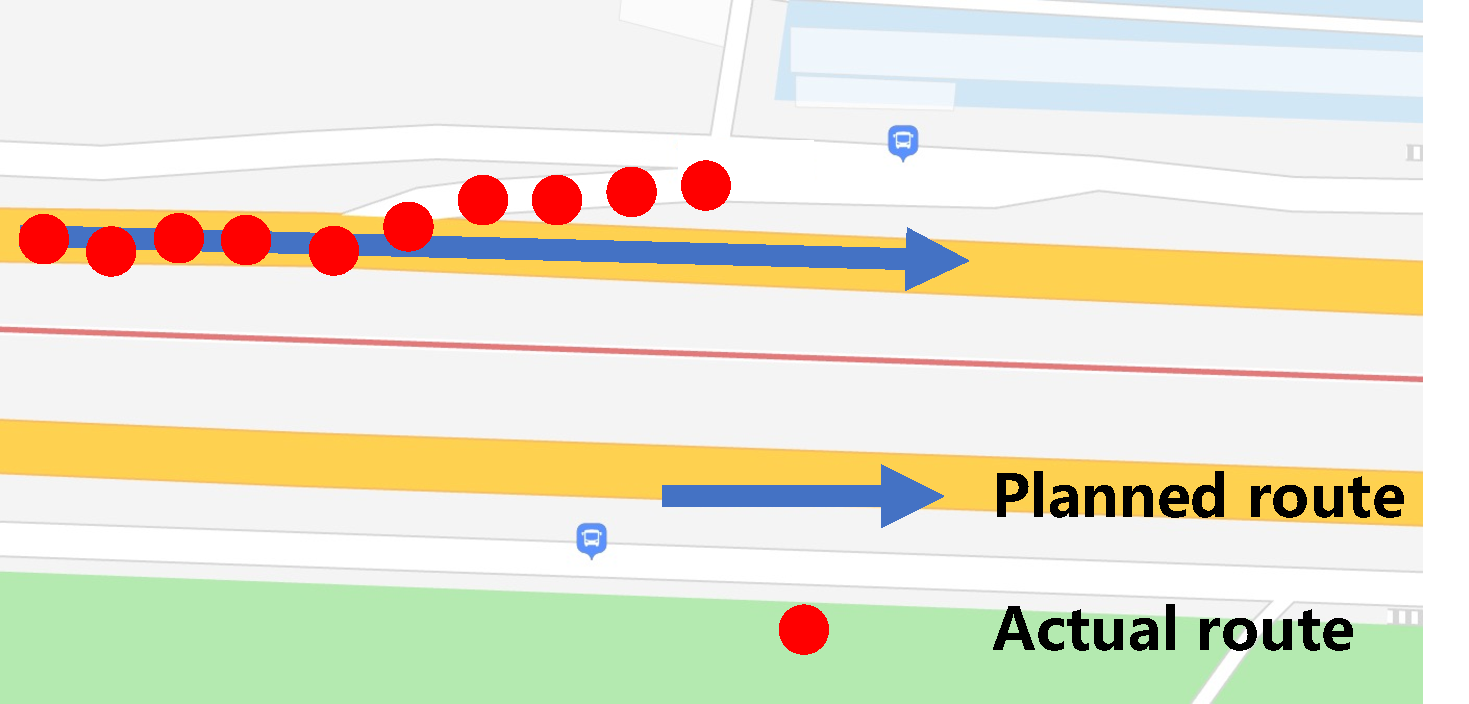
\includegraphics[width=0.4\textwidth]{fig/yawing.pdf}}
%     \caption{The red dots shows the actual route of the vehicle and the blue line shows the planned route of the mobile navigation software.}
%     \label{fig:yawing}
% \end{figure}

\begin{figure}[tp]\centering
    \subfloat[]
    {
        \begin{minipage}{4cm}\centering
        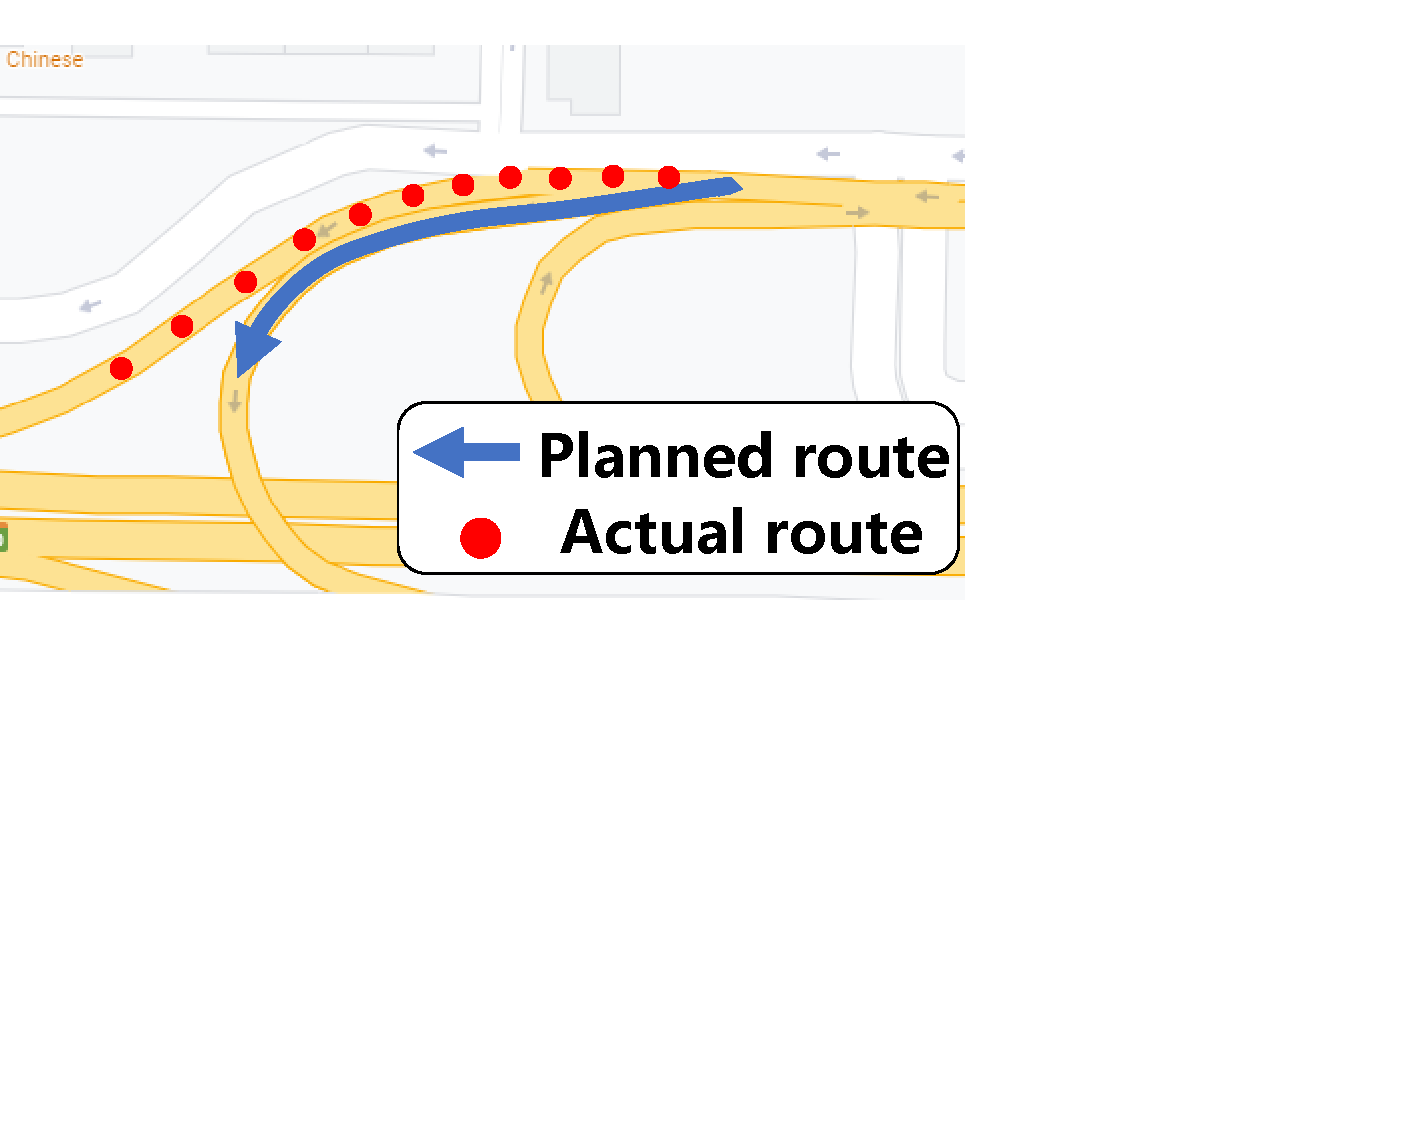
\includegraphics[scale=0.23]{fig/intro_a.pdf}
        \end{minipage}
    }\subfloat[]
    {
        \begin{minipage}{4cm}\centering
        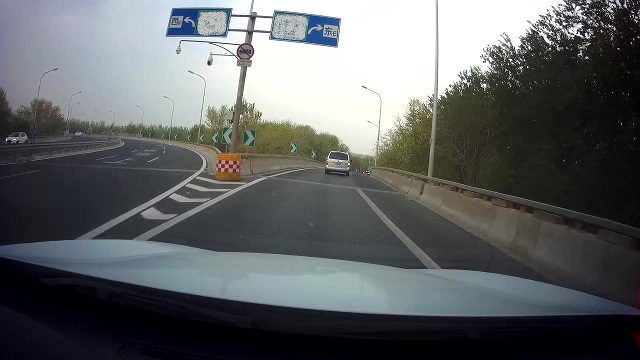
\includegraphics[scale=0.22]{fig/dashcam.jpg}
        \end{minipage}
    }
    \caption{(a) The red dots shows the actual route of the vehicle and the blue line shows the planned route of the navigation application. (b) A fork road image collected by dashcam.}
    \label{fig:intro}
\end{figure}

The most basic and traditional method is map-matching, which locates the vehicle based on GPS signals and road information. But this method is vulnerable to the quality of GPS signal. \cite{gong2015deel} and \cite{won2017hybridbaro} proposed feature-based and barometer-based methods to fetch up the low GPS quality. But these methods still cannot get rid of the influence of the lack of GPS signal.  The latest work, ERNet (elevated road net) \cite{zhang2020elevated}, has leverage deep learning to process the GPS to obtain a more accurate result. However, delay exists in detection. 

% Existing methods for the yawing detection problem, including map-matching, barometer-based, feature-based and ERNet (Elevated Road Network). The map-matching method locates the vehicle based on GPS signals and road information, the feature-based method detects yawing based on satellite signals and IMU data, and the barometer-based method uses the barometer to detect the air pressure to determine whether the vehicle is driving onto an elevated road. ERNet method detects whether a vehicle drive onto an elevated road through a deep learning model. However, the above methods have some problems, such as the accuracy is affected by the GPS signal, the detection delay is long, and the average recognition distance is long.
In this paper, we propose a novel yawing detection framework, which innovatively utilizes image data (shows in Fig. \ref{fig:intro} (b)) to identify the driver's driving intention and uses inertial data to detect vehicle turning to obtain the prediction information of vehicle yawing. Further, we provide real-time and robust yawing detection and tracking by combining these predictions with GPS and road information.\IEEEpubidadjcol

Despite its potentials, a robust yawing detection and tracking system is far from straightforward. First, the road conditions are very complex, and it is difficult to judge the driver's driving intention through the images captured by the dashcam; secondly, effectively fusing multi-source data and apply it to yawing detection is worth considering; finally, the computing power of mobile devices is limited, and the balance between accuracy and operation speed is also a challenge.

In summary, we make the following contributions:
\begin{itemize}
    \item We propose to use images to recognize the driver's driving intention and apply it to the yawing detection scene by adjusting the deep learning model of image recognition to make the yawing detection more robust.
    \item We use the particle filter method based on Monte Carlo framework to fuse data such as image, GPS, and IMU to improve the real-time and effectiveness of yawing detection.
    \item We performed experiments to verify the effectiveness of the method. Results demonstrated that our method can detect 90\% yawing cases in advance correctly.
\end{itemize}

The architecture of our system will be depicted in \ref{sec:overview}.
In section \ref{sec:image}, we will describe the driving intention recognition network.
The system of tracking is presented in section \ref{sec:tracking}.
And section \ref{sec:exp} introduces our experimental design, results, and analysis of the results in detail.

\section{Motivation}
We exposition our consideration on constructing a tracking system to solve the yawing detection issue, including predicting whether the vehicle is yawing in advance, improving the system's efficiency on mobile devices, and integrating multi-source data to make the system more robust.

\subsection{Detection or Prediction}
To detect vehicle yawing effectively, we desire to forecast the driving intention of the vehicle before it enters the fork road. However, GPS cannot give predictions. By observing other sensor data, we discovered that both IMU and image contain predictive information for yawing. In addition, compared to the lane change information from the IMU that does not appear stable, the image can always reveal the road the vehicle is about to enter (e.g. Fig. \ref{fig:intent}). Therefore, as long as images from ubiquitous dashcams are successfully used, we can achieve the predictive ability of vehicle yawing.

\begin{figure}[htbp]
    \centerline{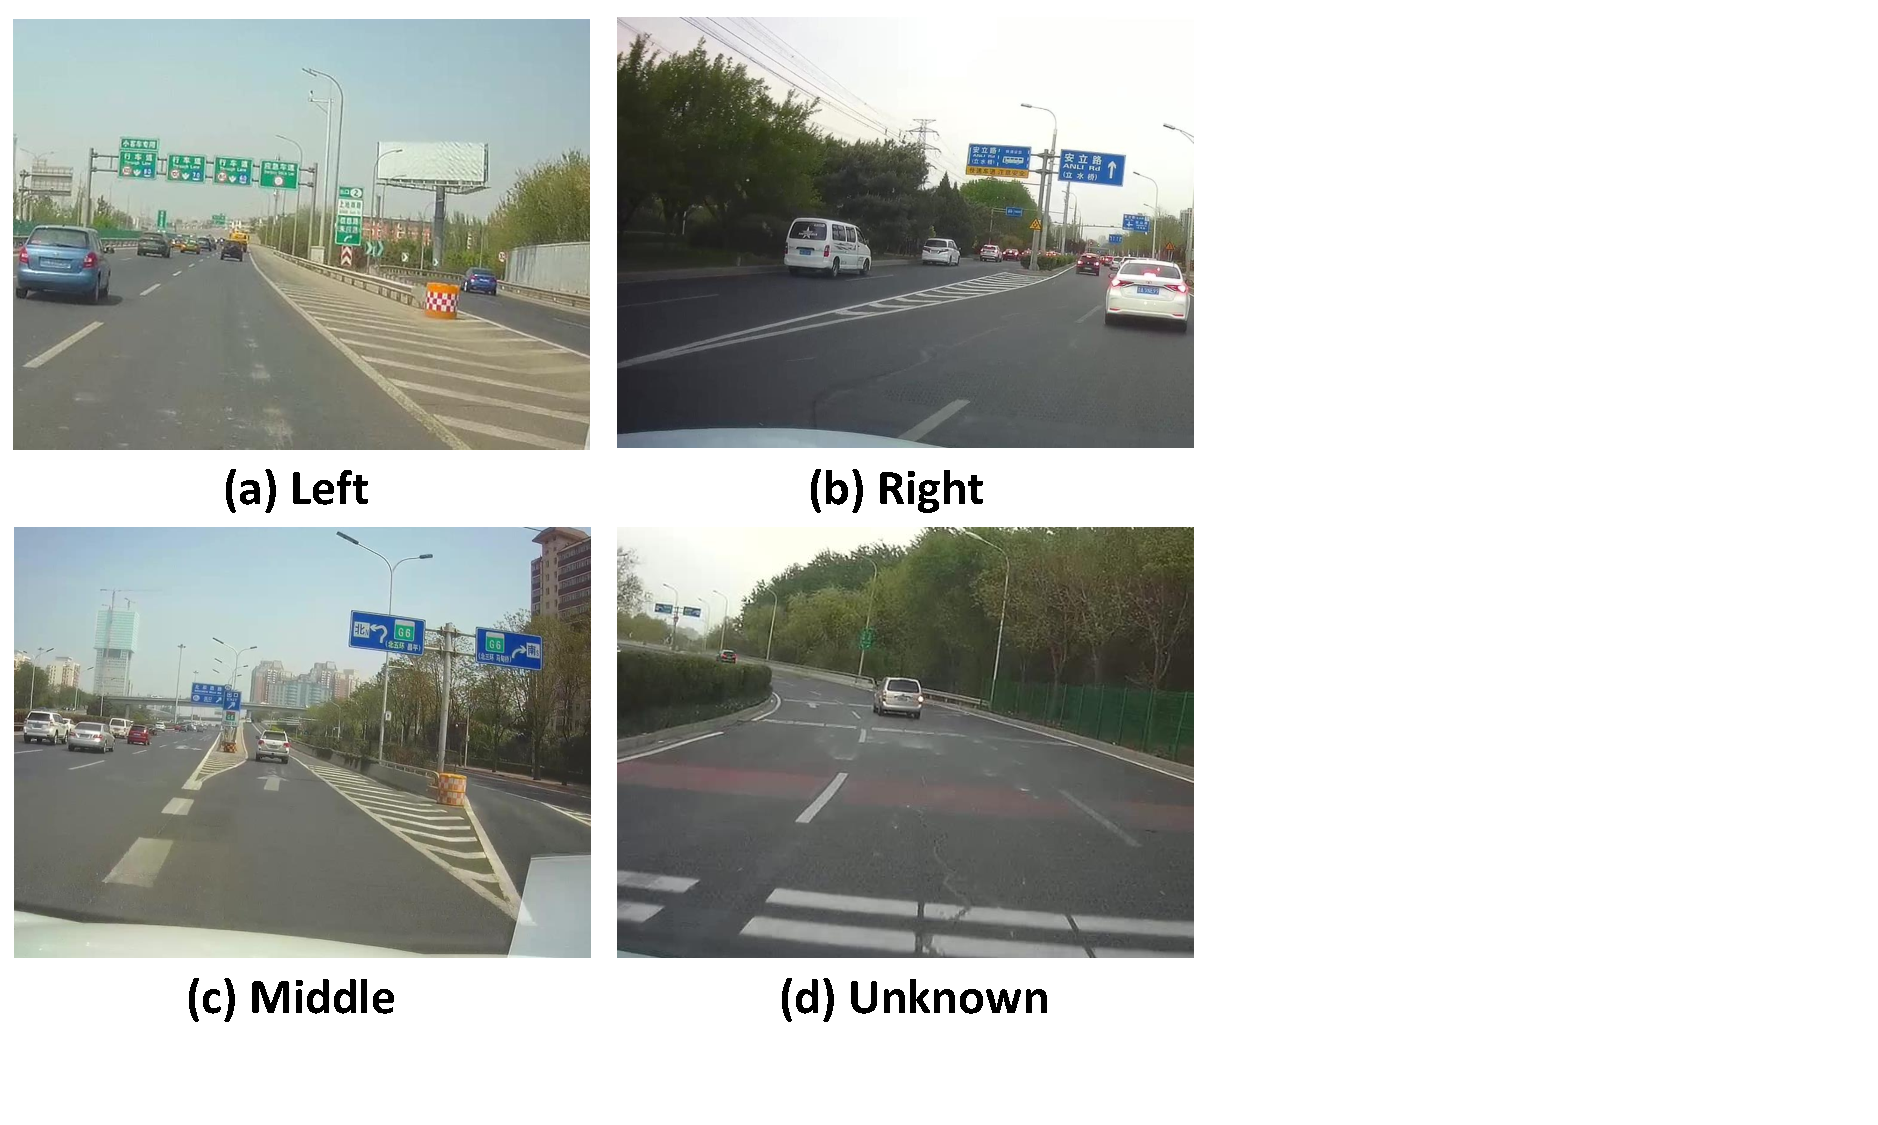
\includegraphics[width=0.5\textwidth]{fig/intention.pdf}}
    \caption{The four images captured by dashcam correspond to the four intentions. }
    \label{fig:intent}
\end{figure}

In fact, Casas et al. \cite{casas2018intentnet} have proposed the prediction of vehicle driving intention through neural network back in 2018. But instead of using several data to predict complicated intentions such as vehicle trajectories, we only need to know which road the vehicle is going. Therefore, we divide the intention into four categories: 

% The driving intention is the learning target of the nerual network and we define as 4 categories: 
% \begin{equation}
    $$Intentions: \{ left, right, middle, unknown\}$$
% \end{equation}
% We describe the driving intention as directions since drivers have to choose one direction to enter when facing a fork road.

As shown in Fig. \ref{fig:intent}, $Left$ means that the vehicle drives towards left when facing to the fork road, and $right$ is opposite. $Middle$ only appears when there are three or more alternative roads, and the vehicle drives towards middle. The most special one is $unknown$ due to the driving intention cannot be clearly understood in some cases. For instance, the driving direction cannot be distinguished when the fork section has not yet reached, or there is something (e.g. other vehicle, tree, etc) blocking the front.

At this point, we define the intention recognition problem as a classification problem, and we can choose dozens of high-precision image encoders, such as Inception \cite{inceptionv3}, ResNet \cite{he2016deep}, Vision Transformer \cite{vit}, MobileNet \cite{mobilenetv3}, etc.
Nevertheless, our system is oriented toward edge devices, such as mobile phones or onboard computing platforms, so we need to balance the accuracy and model computation loss when designing the model.


\subsection{Running on Mobile Devices}

In order to run the intent recognition model as efficiently as possible on mobile devices, we try to compress it. The operation efficiency of the model is mainly affected by the number of parameters and computation:
\begin{itemize}
    \item The number of parameters directly determines the space occupied by the model. The reduction of model parameters allows the model to consume less memory at runtime. In deep learning models, the parameters of the fully connected layer are often very dense.
    \item The computation affects the inference time and power consumption required. The smaller the computation, the less inference time and energy the device costs. In general, convolutional neural networks involve a great deal of computational cost.
\end{itemize}

Previous works have proposed many methods to compress models, such as pruning, knowledge distilling, low-rank factorization, model quantization, etc. In addition, some ingenious architectures (i.e., MobileNet, ShuffleNet) are also the product of the concept of model compression. Among them, many researchers utilize the pruning method because of its convenience. Filter-based pruning methods can reduce device storage usage and decrease computation costs effectively while manageable to deploy. Therefore, based on the selection and design of the small model, we adopt filter-based pruning to compress it further.

However, even though the model could be fast and accurate, it is far from robust to rely only on images for yawing detection.

\subsection{Multi-source Fusion}
We further improve the stability and usability of the system through the fusion of multi-source data. We divide the available data into four parts: images, IMU, GPS, and road information.

\begin{figure}[htbp]
    \centerline{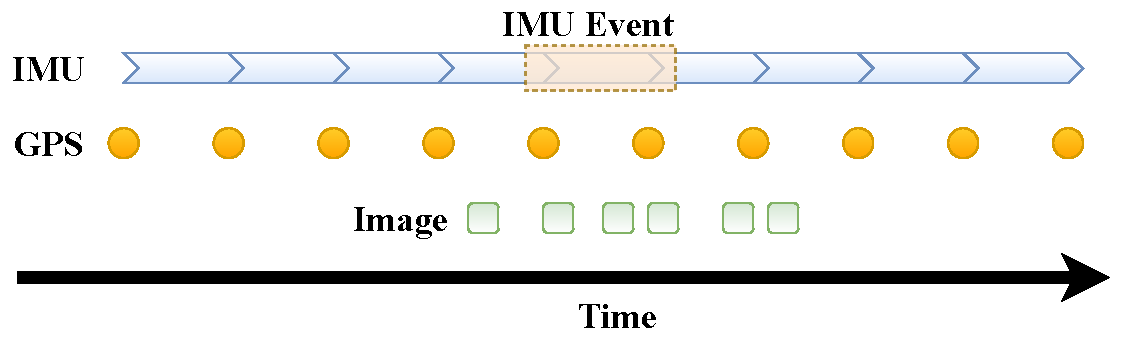
\includegraphics[width=0.5\textwidth]{fig/data_freq.pdf}}
    \caption{The data distribution (except road information) over the time axis. The frequency of the IMU is 50 Hz, the frequency of the GPS is 1 Hz, and the image data is 1-2 Hz. Event detection (lane change) based on IMU data is sometimes unavailable. }
    \label{fig:data_freq}
\end{figure}
\begin{itemize} 
    \item Road information.
    Road number; the longitude and latitude data of the fork point, yawing detection start point which is about 50 meters away from the fork point,  and points on every fork road.
    \item GPS.
    \item IMU.
    \item IMG.
\end{itemize}

Figure. \ref{fig:data_freq} shows the timestamps of different data appearing in a fork tracing process. The GPS and IMU data are continuous, while images are opportunistic. Moreover, the lane change information obtained from the IMU is even more unstable since lane-changing behavior does not always exist. 

\section{System Overview}\label{sec:overview}
This paper proposes an accurate and real-time tracking framework for yawing detection.
% Even when elevated overlaps and fork roads are too close, it can also achieve good results. 
Fig. \ref{fig:SystemOverview} shows our system architecture.

\begin{figure}[htbp]
    \centerline{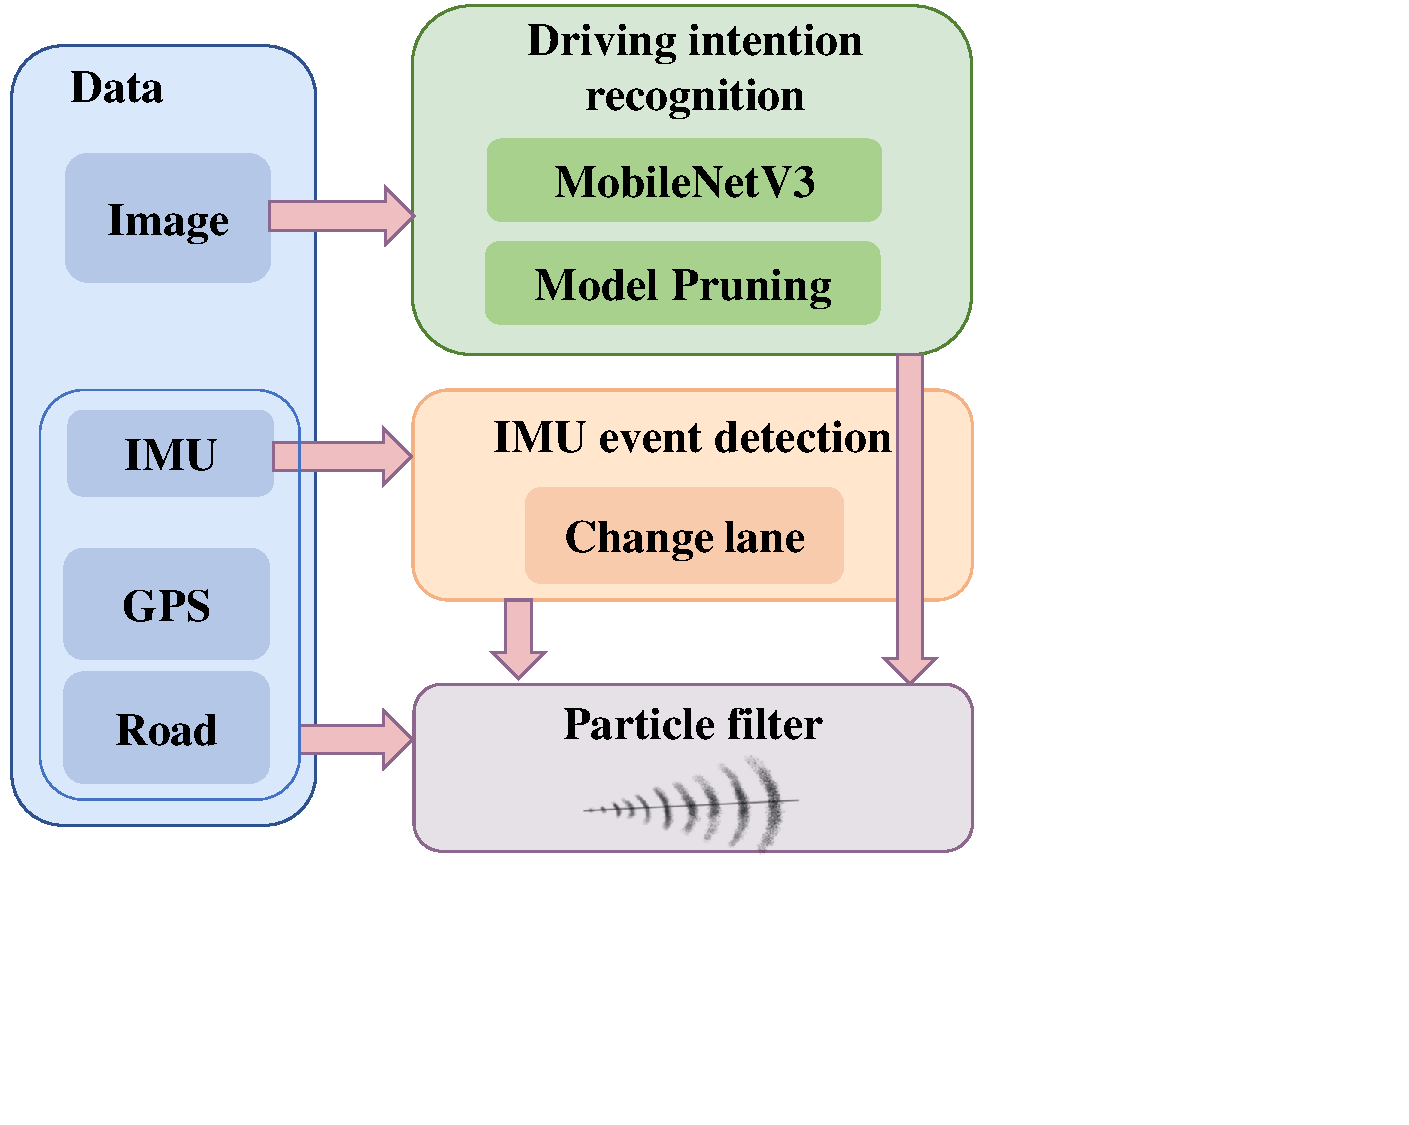
\includegraphics[width=0.5\textwidth]{fig/SystemOverview1.pdf}}
    \caption{System Overview}
    \label{fig:SystemOverview}
\end{figure}

First, when the vehicle is driving on a normal road, the map-matching method is used to locate the vehicle through GPS and road information. When meeting a fork road, our system will input the image captured by the dashcam into the deep learning model to predict the driver's driving intention. At the same time, we will use IMU event detection to determine whether the vehicle changes lanes. Finally, the particle filter fuses the IMU event detection and driving intention results with GPS and road information to track the vehicle and predict whether it is yawing.
% In the following sections, we will explain them in sequence.

\section{Fork Tracker}
% \section{Driving Intention Recognition}\label{sec:image}
\subsection{Driving Intention Recognition}\label{sec:image}
We utilize a deep learning model to predict the driver's driving intention via the picture collected from the dashcam.
In this section, we design a model that can learn the driver's driving intention from a single image.

\begin{figure*}[htbp]
    \centerline{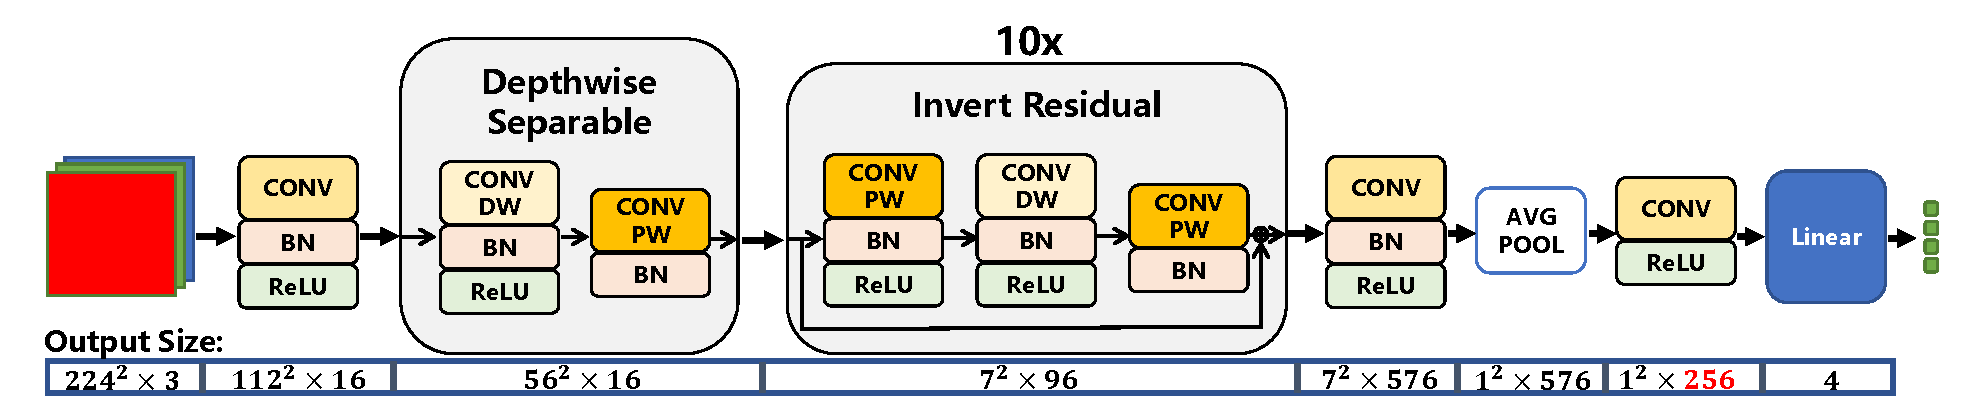
\includegraphics[width=1\textwidth]{fig/net.pdf}}
    \caption{Model architecture. Input data is a single RGB image. The data dimension is increased by the first layer of convolution to avoid the problem of information loss due to ReLU and low dimension as \cite{mobilenetv2} proposed. Then the \textit{Depthwise Separable convolution} \cite{howard2017mobilenets} block encode the features, which effectively reduces the parameters but maintains high accuracy. And \textit{Invert Residual} \cite{mobilenetv2} blocks increase the expressiveness of nonlinear per-channel transformations by connecting the input and output. Note that only if input and output have the same number of channels can they be connected. Finally, features are processed into the four outputs by an efficient encoder \cite{mobilenetv3}. }
    \label{fig:net}
\end{figure*}
 
% Because the model runs on mobile devices, it needs to be lightweight.
% \subsection{Driving intention}

Our network is designed based on MobileNetV3 \cite{mobilenetv3}, which has been proven to be a very effective image classification network. 
% MobileNetV3 is a very lightweight convolutional neural network with a good performance on mobile devices. 
In addition, \cite{mobilenetv3} defines the net of two scales: large and small. The small one is targeted at lower resource. Based on MobileNetV3-Small, we carried out adaptive parameter optimization and compression. On the premise of ensuring the accuracy, we reduced the number of parameters of the model to improve the computational efficiency. The model structure is shown in the Fig. \ref{fig:net}.

Compared to MobileNetV3 \cite{mobilenetv3}, we abandon the \textit{Sqeeze-and-Excite} \cite{hu2018squeeze} block and \textit{h-swish} nonlinearity activation function since they introduce computation but few improvements in our problem.  
Moreover, we modify the channels from 1024 to 256 in the last convolution layer which can significantly reduce the number of parameters but with only a slight loss of accuracy in our system. Detailed evaluation will be shown in the experiments section.
\subsection{Model Compression}\label{sec:pruning}
According to the prediction of driving intention and the fusion of multi-source sensor data, we construct a yawing detection system based on sequential Monte Carlo (Particle filter). However, during the real-world experiments, we found that the performance of driving intention detection model is far from that when using local datasets, and has a negative impact on the accuracy of the final results of the whole system. This is because the calculation time of intention model is too long, so the information given by the image cannot be fed back to the system in time. Different from the dataset with a given timestamp, the state of the vehicle is always changing, and the decision given by the system comes from the state of the previous moment. Moreover, the system includes IMU, GPS and other source data with different observation frequencies, when fusing through particle filter, we need to align their timestamps. Therefore, the performance of the system depends on the consistency between the given decision and the real state. Training a compressed model to improve the efficiency and the prediction accuracy is very important for the optimization of the model.

The main methods of model compression are model distillation, quantization and pruning. Model distillation uses a small model to learn a large model with a sparse network through knowledge transfer, and finally obtains a lightweight model; model quantization reduces the accuracy of some parameters in the trained model to achieve the effect of model compression; model pruning sorted the parameters according to the importance of norm or weight, and the parameters with low importance are set to zero or directly pruned.

The common method of model pruning is to fine-tune the trained model. It will sort the weights of its convolutional layer parameters and set the lower weights to zero or calculate the norm of the convolutional layer filter and remove smaller one. However, these methods produce other problems. Although they improve the efficiency of the model, the accuracy will decrease greatly. The prediction of driving intention is the main data source in this system, so the decrease of its accuracy will directly influence the prediction accuracy of the system at the same time.

\begin{figure}[htbp]
    \centerline{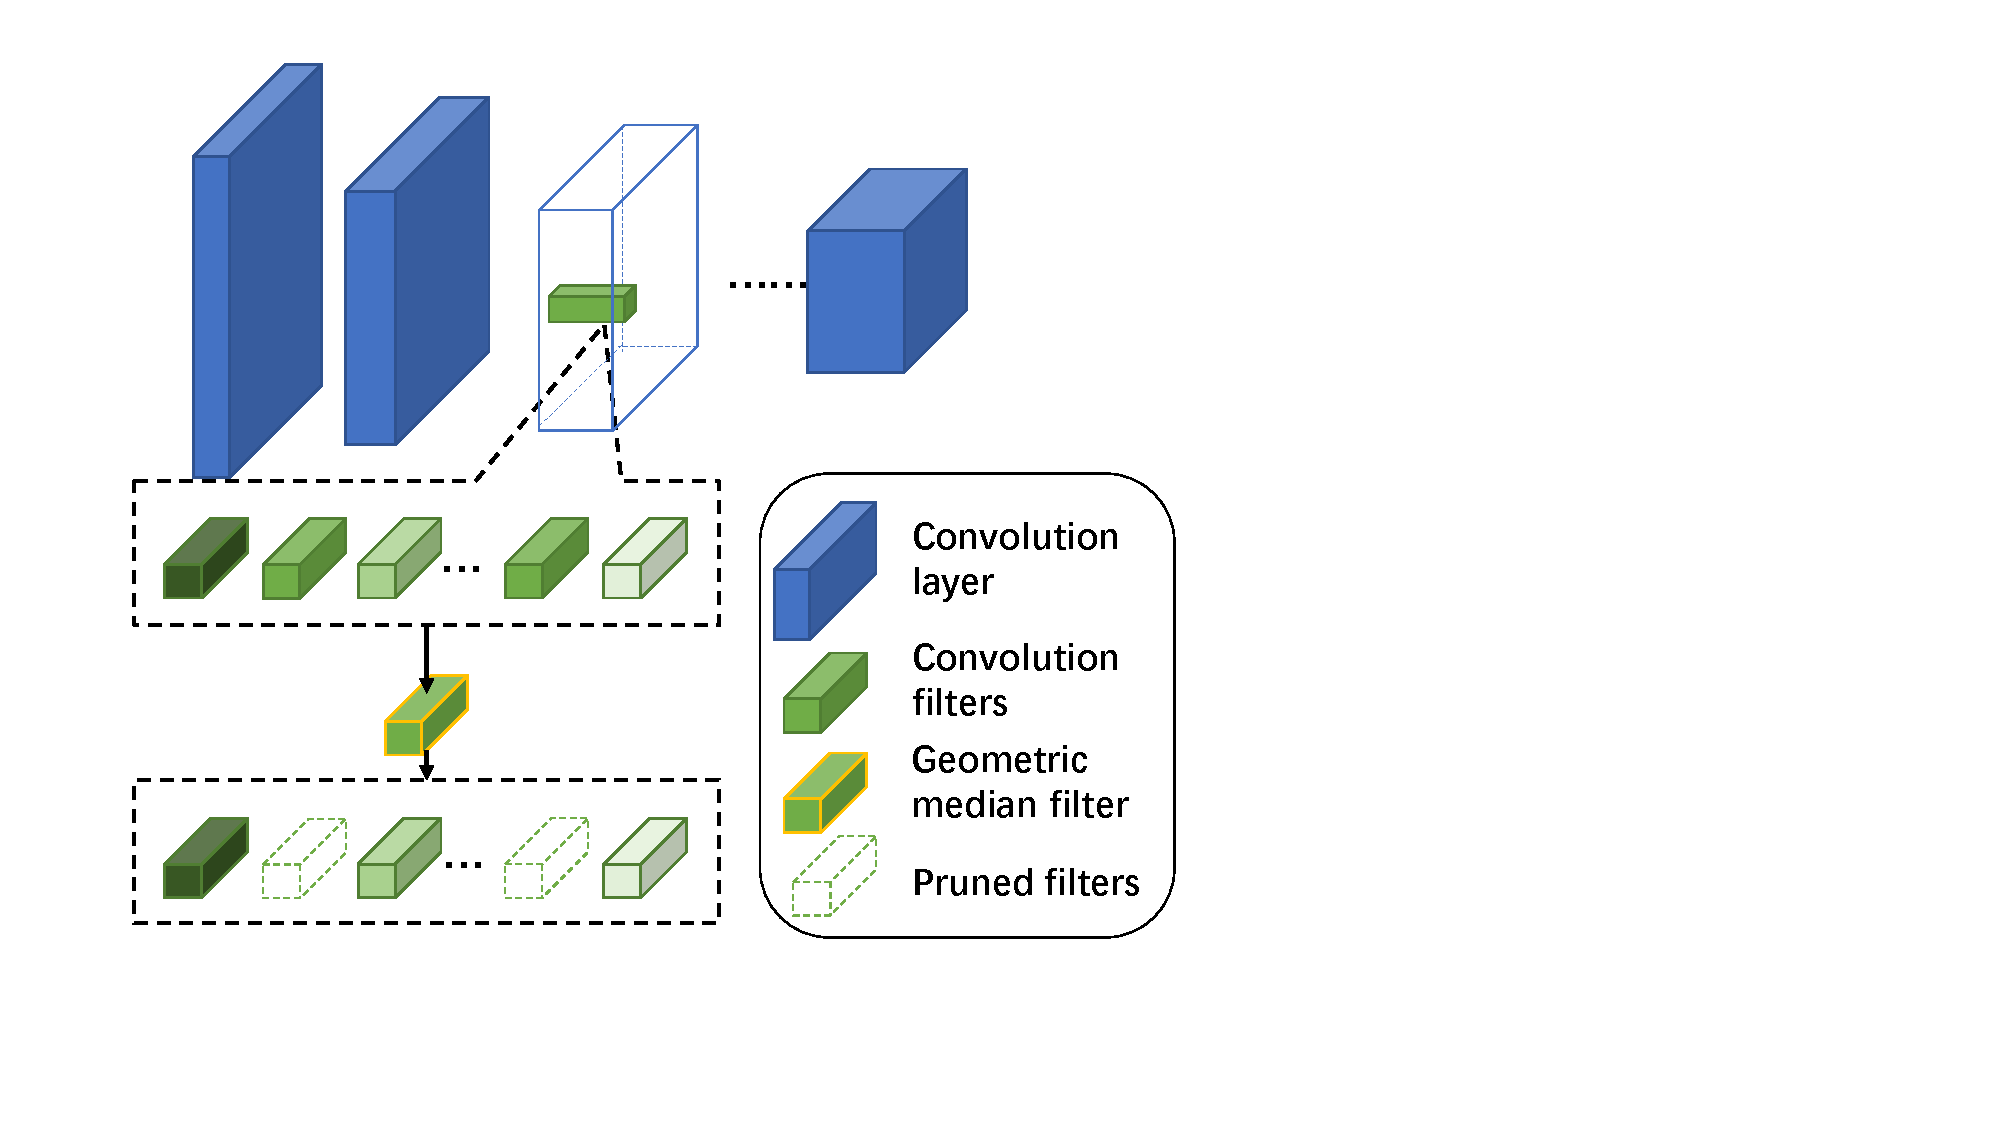
\includegraphics[width=0.5\textwidth]{fig/model_pruning.pdf}}
    \caption{Pruning via Geometric Median.}
    \label{fig:pruning_median}
\end{figure}

To solve the above problems, we propose the filter pruning method based on geometric median points and combine it with our application scenarios. Through our experiments, it can be proved that while improving the efficiency of the model, it can achieve an accuracy approach to the data set experiment. The basic idea is to synchronize the model pruning with the model training process and complete it by calculating the geometric median point. In addition, this method no longer clips filters, but performs a zeroing operation, and the clipped filter will still participate in the training of the next epoch in its complete form. Such a pruning method can reduce the norm restriction of the filter, and make the pruned model still maintain a high learning ability to avoid performance degradation. Pruning is performed after each epoch training. The specific steps are as follows: 
\begin{enumerate}
  \item 
  Obtain all convolutional layers that need to be pruned and the pruning rate.       
  \item 
  Calculate the Euclidean distance of all filters in the convolutional layer, and obtain the Euclidean distance Geometric median point. 
  \item 
  Set all parameters of filters close to the geometric median point to zero; then, the model will continue to train for the next epoch.
\end{enumerate}

\subsection{Tracking}\label{sec:tracking}
Beside the intention recognition from images, another core of our system is fusing multi-source data\cite{hostettler2014vehicle} to obtain a more accurate vehicle trajectory. We first briefly describe the Monte Carlo framework we apply, then demonstrate the input to the system, and finally introduce the yawing detection and tracking system we designed in detail.

\subsubsection{Data Processing}
\textbf{Inertial sensors. }
Our method mainly uses the data of gravity sensor, acceleration sensor and gyroscope sensor inside the mobile phone to estimate the driving trajectory of the vehicle. We transform the mobile phone coordinate system to the car coordinate system \cite{xiao2021many, gao2017smartphone}, and the vehicle trajectory can be obtained by $\Vec{x(t)}=\iint\Vec{a(t)}\mathrm{d}t$. We use the sliding window to detect the vehicle turning events. The window will obtain the change of the z-axis of the gyroscope in a period of time, and then we calculate the difference between the maximum and minimum points in the window. When the midpoint of the window is at the extreme point and the extreme point difference is greater than the threshold, the action of the vehicle is identified as a turn and will be marked. Turning detection is mainly used for yawing recognition in fork road scenes.

\textbf{GPS and road information.}
When people drive the car, the smartphone will continuously collect GPS data such as longitude and latitude, and the collected GPS data will form the trajectory of the vehicle. The system will project the GPS points to the best matching road in sequence (As shown in Fig. \ref{fig:projection}) and combine GPS data with road information. When the system detects that the distance between the GPS point position and the starting point of the elevated or fork road is less than a certain value, the yawing detection is triggered.

\begin{figure}[htbp]
    \centerline{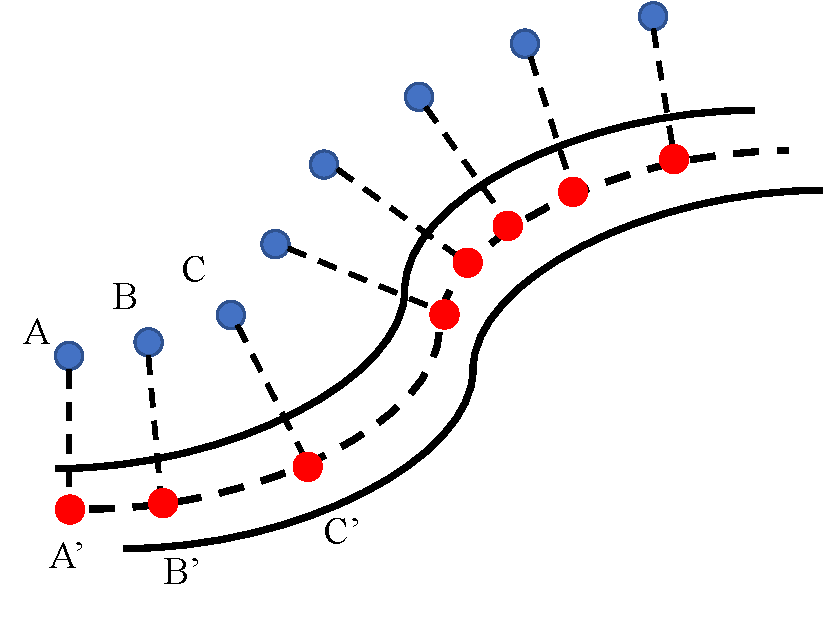
\includegraphics[width=0.3\textwidth]{fig/projection.pdf}}
    \caption{The blue point is the GPS point, and the red point is the projection point.}
    \label{fig:projection}
\end{figure}

\textbf{Image prediction result.}
We improve the confidence of image prediction results (described in \ref{sec:image}) by reducing recall instead of directly using them. 
In a tracking process, only a few images are needed to have a key impact on the tracking results. But the whole tracking process often obtains several image prediction results. Therefore, we filter each prediction result by setting a threshold. If for an image, the model's prediction probabilities for all classes are lower than the threshold, then we consider the model's output to be invalid. Doing so reduces the recall of the model output, but increases the confidence of the predictions.

\begin{figure}[htbp]
    \centerline{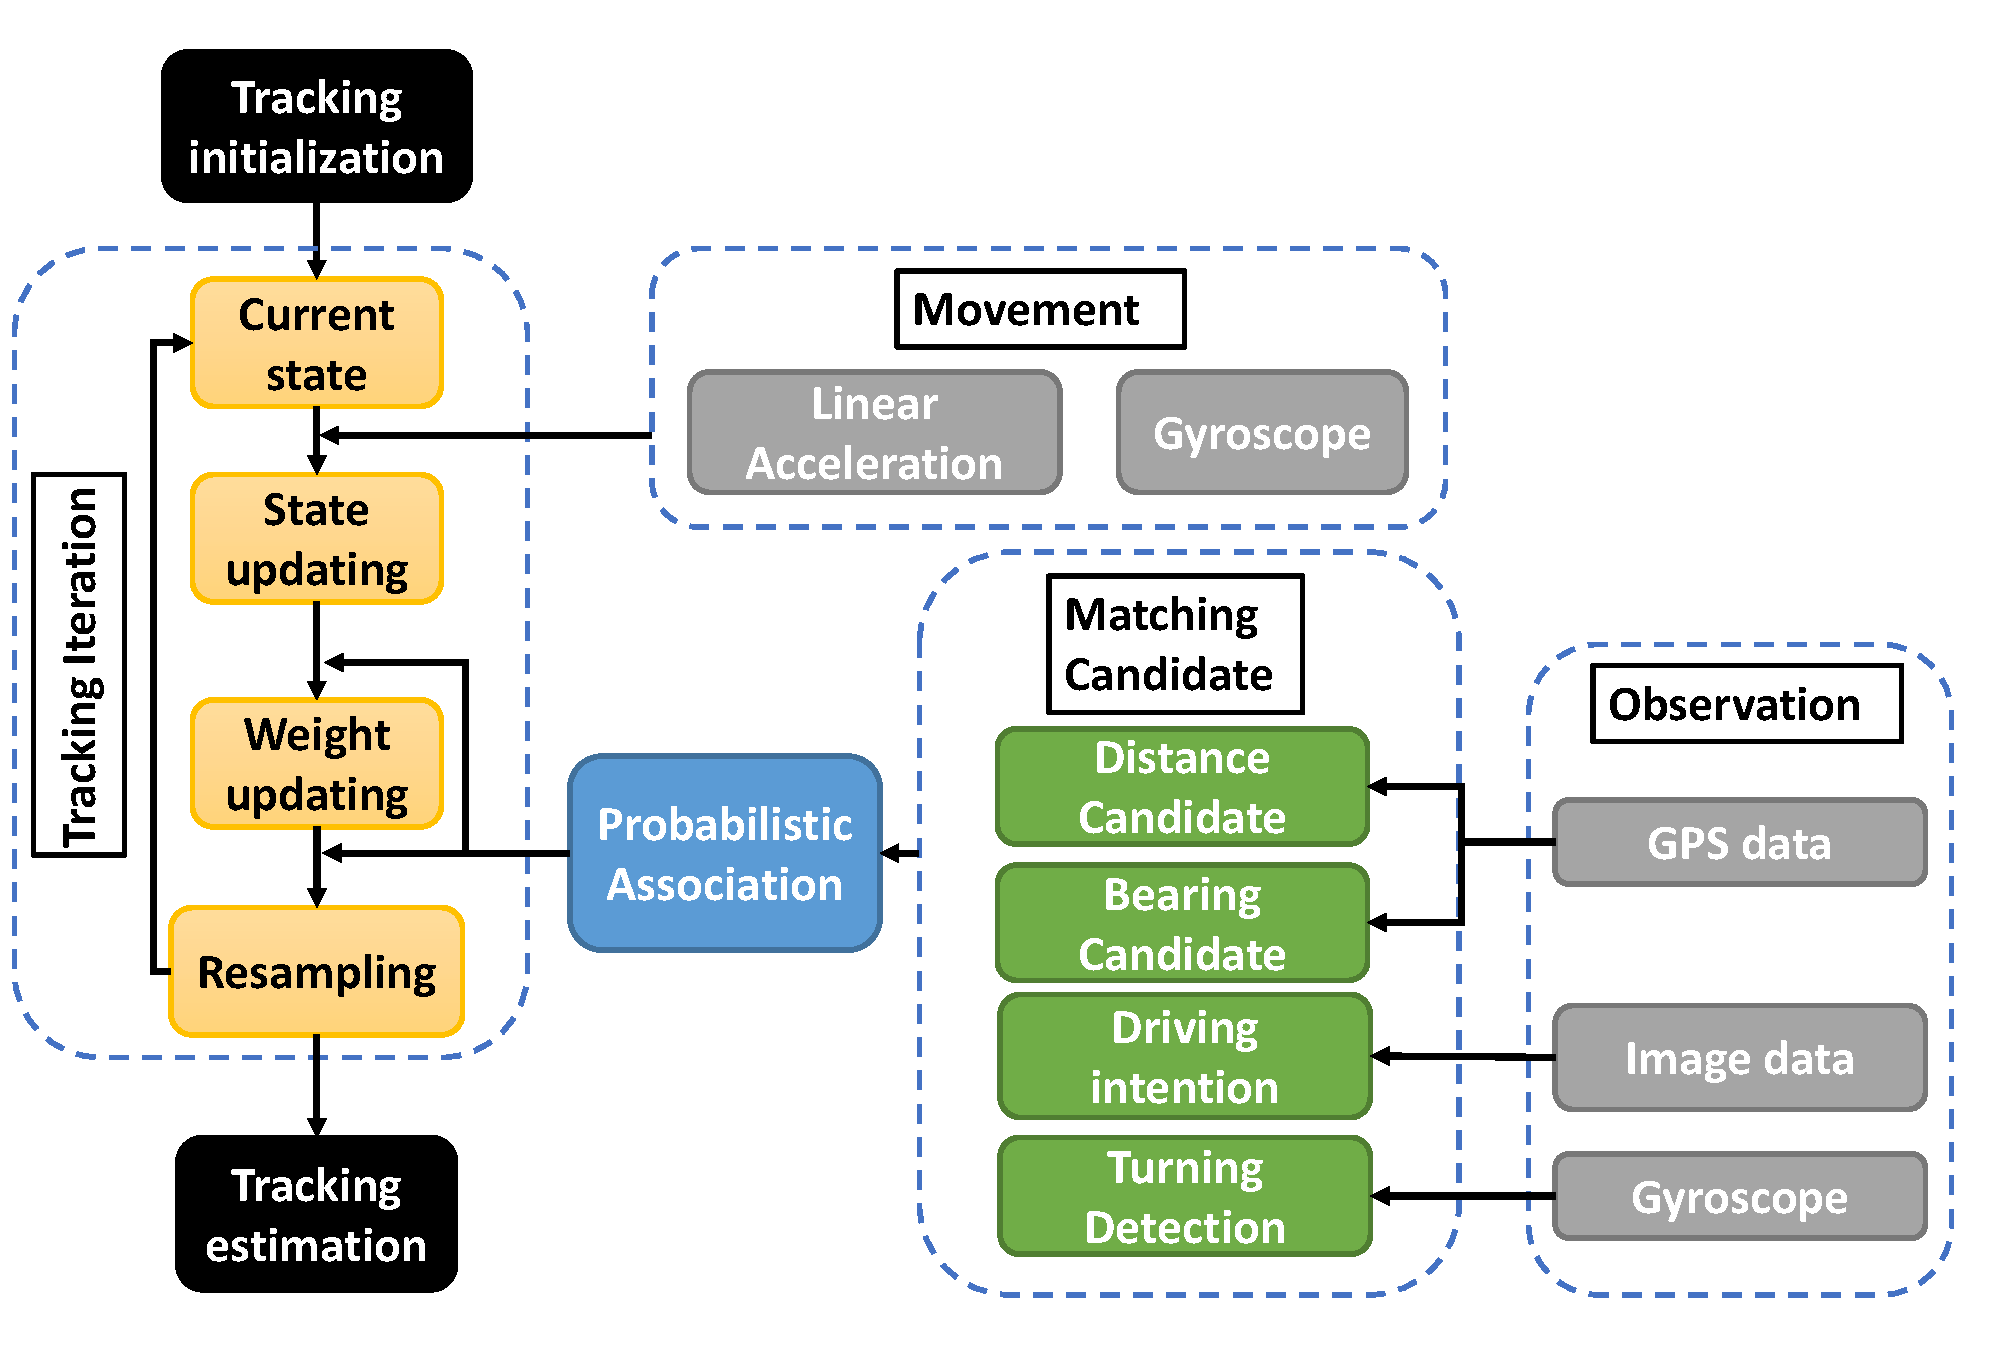
\includegraphics[width=0.48\textwidth]{fig/PF-Systemoverall.pdf}}
    \caption{An overview of Tracking system.}
    \label{fig:track_system}
\end{figure}

\subsubsection{Probabilistic Tracking Framework}
 We use probabilistic estimation method to estimate the location distribution of the vehicle. Because the measurement errors and noises of different sensors are complex and do not necessarily obey the Gaussian distribution, linear filtering is difficult to solve the problem. Therefore, we adopt a trajectory inference method based on sequential Monte Carlo (i.e., particle filtering). It uses N particles that contains multi-dimensional vectors to represent the state probability distribution of the car at the current time t, and iterate continuously through the following three steps\cite{du2019enhanced}:

\textbf{State update.} 
The particle state estimation $\hat{S}_{t}^{(N)}$ at time $t$ is obtained from the set of particle states $\hat{S}_{t-1}^{(N)}$ at the previous time and the movement at the current time. It includes obtaining the position at time $t$ by $v_{t-1}$ and obtaining the velocity $v_{t}$ at time $t$ by $a_{t}$ and other state estimations.

\textbf{Weight update.}
The likelihood probability $p(z_{1:m,t}|\hat{s}_t)$ obtains from the measurement value $z_{1:m,t}$. Then the system adjusts the weight of each particle to provide a larger weight for those who has a higher likelihood $p(z_{1:m,t}|s_t = \hat{s}_t)$. Finally, the weights $\omega_{t}^{n}$ are normalized to the same scale, and particles $\hat{S}_t$ at time t is formed.

\textbf{Resampling.}
To prevent weights from gradually concentrating on a small number of particles (particle degradation), the particle set $S_{t}^{N}$ is resampled after each iteration. We will get a new particle set $S_{t}^{N}$ by random sampling and set all particle weights to be the same $\omega_{t}^{n} = \frac{1}{N}$.

% Next, we explain how to fuse the data in detail .
% \subsection{Input}

% \subsection{Tracking Algorithms}

\subsubsection{Initialization and update}


First, we will initialize the particle state based on the prior knowledge of the trigger point. Each particle has a state $(lat_{t},lon_{t},v_{t},\beta_{t},rid_{t},p_{r,t},p_{l,t})$, The latitude and longitude of the particle $lat, lon$, the initial speed $v$, the heading angle $\beta$ and the maximum possible road information $rid$ will be directly given by the GPS information of the trigger point, and the right turn and the left turn probability will be initialized to $\frac{1}{2}$.


The particle state $(lat_{t-1},lon_{t-1},v_{t-1},a_{t-1},rid_{t-1},p_{r,t-1},\\
p_{l,t-1})$ at time t-1 will update according to the state equation and the IMU state $m_t=(a_y,\omega_z)$. $(\hat{lat}_t,\hat{lon}_t)$ is updated through:
\begin{equation}
\Delta{d} = v_{t-1}\Delta{t}+\epsilon_v
\end{equation}
\begin{equation}
(\hat{lat}_t, \hat{lon}_t) =(lat_{t},lon_{t})+f(\Delta d)
\end{equation}
where $f(*)$ refers to the longitude and latitude change that is converted from moving distance.


Road information $\hat{rid_t}$ is updated through:
\begin{equation}
    \hat{rid_t}=h(\hat{lat}_t,\hat{lon}_t)
\end{equation}
where $h(*)$ refers to a map-matching algorithm combines the road information acquisition with a driving probability.


Velocity $\hat{v}_t$ is updated through:
\begin{equation}
    \hat{v}_t=v_{t-1}+a_{y}\Delta t+\epsilon_v
\end{equation}

Heading direction $\hat{\beta}_t$ is updated through:
\begin{equation}
    \hat{\beta}_t=\beta_{t-1}+\omega\Delta t+\epsilon_\beta
\end{equation}


The probabilities of left and right turn $(\hat{p}_{l,t},\hat{p}_{r,t})$ is updated through:
\begin{equation}
    \hat{p}_{l,t}=\gamma \hat{p}_{l,t-1}+\epsilon_p
\end{equation}
\begin{equation}
    \hat{p}_{r,t}=\gamma \hat{p}_{r,t-1}+\epsilon_p
\end{equation}
where $\gamma$ depends on the characteristic of $\omega$.

Note that, all the $\epsilon$ are the Gaussian noise in these estimation processes.


\subsubsection{Weight update}
The weight of particles will be affected by GPS information, IMU event detection, image observation information and heading angle constraints. The main principle is to reduce the weight of particles that violate the above constraints\cite{gao2017smartphone}. The final weight of the particle is:
\begin{equation}
    \omega _{t} =\prod_{i=0}^{k}\omega_{i,t} 
\end{equation}
Each kind of observation information will be obtained randomly, and k is the number of observations obtained at the current time t. Among them, the equation of $\omega_{i,t}$ can be described as:
\begin{itemize}
    \item Heading angle constraint: According to the limit value of the heading angle change of the car at the current update frequency, we define $\omega _{0} =\cos^{2} (\beta _t-\beta_{t-1})$ to punish the particles whose heading angle mutates.
    \item GPS information constraint: When the GPS information is obtained, according to the distance between the particle and the GPS point, $1/D(lat_t,lon_t,lat_g,lon_g)$ is used to punish the distance Particles with farther GPS points and give awards to others, where  $D(lat_t,lon_t,lat_g,lon_g)$ is the distance between two longitudes and latitudes.
    \item IMU and image constraint: The image will give the prediction information that the current position is towards left, middle or right road, and the IMU event detection will judge the current state of turning left, right and going straight. Therefore, when the image or event information is obtained, we will punish the corresponding particle according to the image information combined with the state of $p_l,p_r$ in the particle. Penalize particles whose driving probability p is opposite to the information given by the image in the manner of $\omega_k=\alpha(1-p),(k=2,3)$, where $\alpha$ is the scale of the punishment.
\end{itemize}

Finally, the normalization formula of all particles are as follow,
\begin{equation}
    \omega=\frac{\omega-\omega_m{}_i{}_n}{\omega_m{}_a{}_x-\omega_m{}_i{}_n}
\end{equation}

We implemented particle filter based method to fuse multi-source data to track vehicles accurately and detect yawing. First, we will initialize the particle states. Next, we update them based on image, GPS, and IMU data, and finally resampling. The experimental results show that the method can achieve accurate vehicle tracking.

\section{Implementation on Mobile device}
In our system, the deep learning model will be deployed on the mobile phones. Since the format of the images captured by the dashcam does not match the requirement of the model input, we use the OpenCV library to process them. The size of the captured image is 1920*1080 pixels. After converting from BGR format to RGB format, resize, and dimension transformation, the image is finally processed into shape of [3,224,224]. In addition, we need to export the model structure and parameters, and load the model on the Android devices through the torch mobile framework. After loading it successfully, the image will be imported into the model and the model will obtain the output for judging the driver's driving intention.

We measured the time occupied by the image processing part and the model running part of the code. We found that the image processing time was longer than the model running time. The image processing time basically does not exceed 100ms, and the model running time does not exceed 60ms. We tested with 20 images, the average image processing time was 72ms, the average model running time was 43ms, and the average total time was 115ms. We also used the image processing tool of Android to process images for comparative experiments and found that the image processing toolkit takes an average of 450ms to process an image. Therefore, it is proved that our image processing method is more time-saving.

\section{Experiments}\label{sec:exp}
\subsection{Dataset}
Our dataset consists of two parts: image data for training the deep learning model and multi-source data for testing our whole system.
\subsubsection{Image data}
Our sufficient image data is collected by the DiDi platform. Dashcams deployed in vehicles occasionally upload captured images, and the large number of ride-hailing vehicles ensure a large data source. 
But we still have to label these quantities of data to train the nerual network, so we implement a semi-auto label workflow. The workflow can be divided into two steps: reversely deduce the label based on the completed trajectory, and manual verification. We extract the image near the fork road and label it according to the road information and the trajectory. Then verify these images manually. Note that it is necessary to manually pick out pictures that cannot distinguish the direction which should be labeled as unknown.
Ultimately, we construct a dataset of 21,089 images, of which 7,335 are left, 3,342 are right, 10,000 are unknown, and 412 are middle.
\subsubsection{Multi-source data}
These data are used to evaluate the system and we collect them by driving vehicles ourself. As discussed in Sec. \ref{sec:tracking}, these data must include both GPS, IMU, and imagery, and they must also be able to be time-stamped aligned. 
We collected more than 20 hours of data, including the driving data of three vehicles. Each sequence includes 1 Hz GPS and 50 Hz IMU data collected by the smartphone while driving, as well as 2 Hz dashcam image data. And we finally manually log the yawing result for each sequence.
\subsection{Driving intention recognition}
We evaluate our driving intention recognition model separately. 
We will first introduce the training details, and then compare and evaluate our model with other models in terms of accuracy and parameter quantity.
\subsubsection{Training details}
In implementation, we use PyTorch to train our model on the machine learning platform with one GeForce GTX 2080 Ti GPU, an Intel i7 CPU and 40G RAM. The ratio for training/validation/test split is 7:1:2. 
We set the batch size of 64 and train the model for 200 epochs using Adam optimizor with initial learning rate of 2e-3 and learning rate decay rate of 0.1 every 30 epochs. All our models train based on the pretrained model of Imagenet.
In addition, we implement EMA (Exponential Moving Average) to improve the final performance of our model. 
\subsubsection{Performance}
Table \ref{tab:performance} shows the performance of different network on our image dataset. Normally, we count the total number of MACs (Multiply-Accumulate Operations) and parameters. From Table \ref{tab:performance} we can find our models have significant drop in the number of parameters and storage, while sacrificing only a little accuracy compared to other models. The difference between \textit{Ours-128} and \textit{Ours-256} is the output channels of last convolutional layer, set to 128 and 256 respectively. Relative to the slight reduction in MACs and Params, there is a 0.9\% drop in accuracy, which we think is not worth it, thus we choose \textit{Ours-258} as our final model.
\begin{table}[htbp]
    \centering
    \caption{Performance of different network}
      \begin{tabular}{c|c|cc|c}
      \toprule[2pt]
      Model & {Top1-Acc} & {Params} & {MACs} & {RAM} \\
      \midrule
      AlexNet & 75.2  & 57M   & 710.3M & 217MB \\
      InceptionV3 & 80.2  & 21M   & 2.86G & 83MB \\
      MobileNetV3-large & \textbf{83.5} & 4.2M  & 224.2M & 16MB \\
    MobileNetV3-small & \textcolor[rgb]{ .267,  .447,  .769}{81.4} & 1.5M  & 62.6M & 5.8MB \\
      \midrule
    Ours-256 & 80.8  & \textcolor[rgb]{ .267,  .447,  .769}{0.57M} & \textcolor[rgb]{ .267,  .447,  .769}{57.9M} & \textcolor[rgb]{ .267,  .447,  .769}{2.2MB} \\
      Ours-128 & 79.9  & \textbf{0.5M} & \textbf{57.8M} & \textbf{1.9MB} \\
      \bottomrule[2pt]
      \end{tabular}%
    \label{tab:performance}%
  \end{table}%

However, results in Table \ref{tab:performance} only show the Top1-Acc in a traditional way. In our tracking system, we try to reduce the recall to enhance the accuracy of the intention recognition. 
Since the output of the model is the probability of each class (right, left, middle, unknown), the traditional measurement method is to take the class with the highest probability, such as Top1-Acc or Top5-Acc. 
In our system, we set a threshold to improve the validity of results. We consider the output with the maximum probability less than the threshold as invalid.
% By setting a threshold, we consider the output with the maximum probability less than the threshold as invalid one, so we can improve the validity of the model system output. 
But this comes at the expense of recall, so we conduct an experiment to explore the changing relationship between accuracy and recall in our system.

\begin{figure}[htbp]
    \centerline{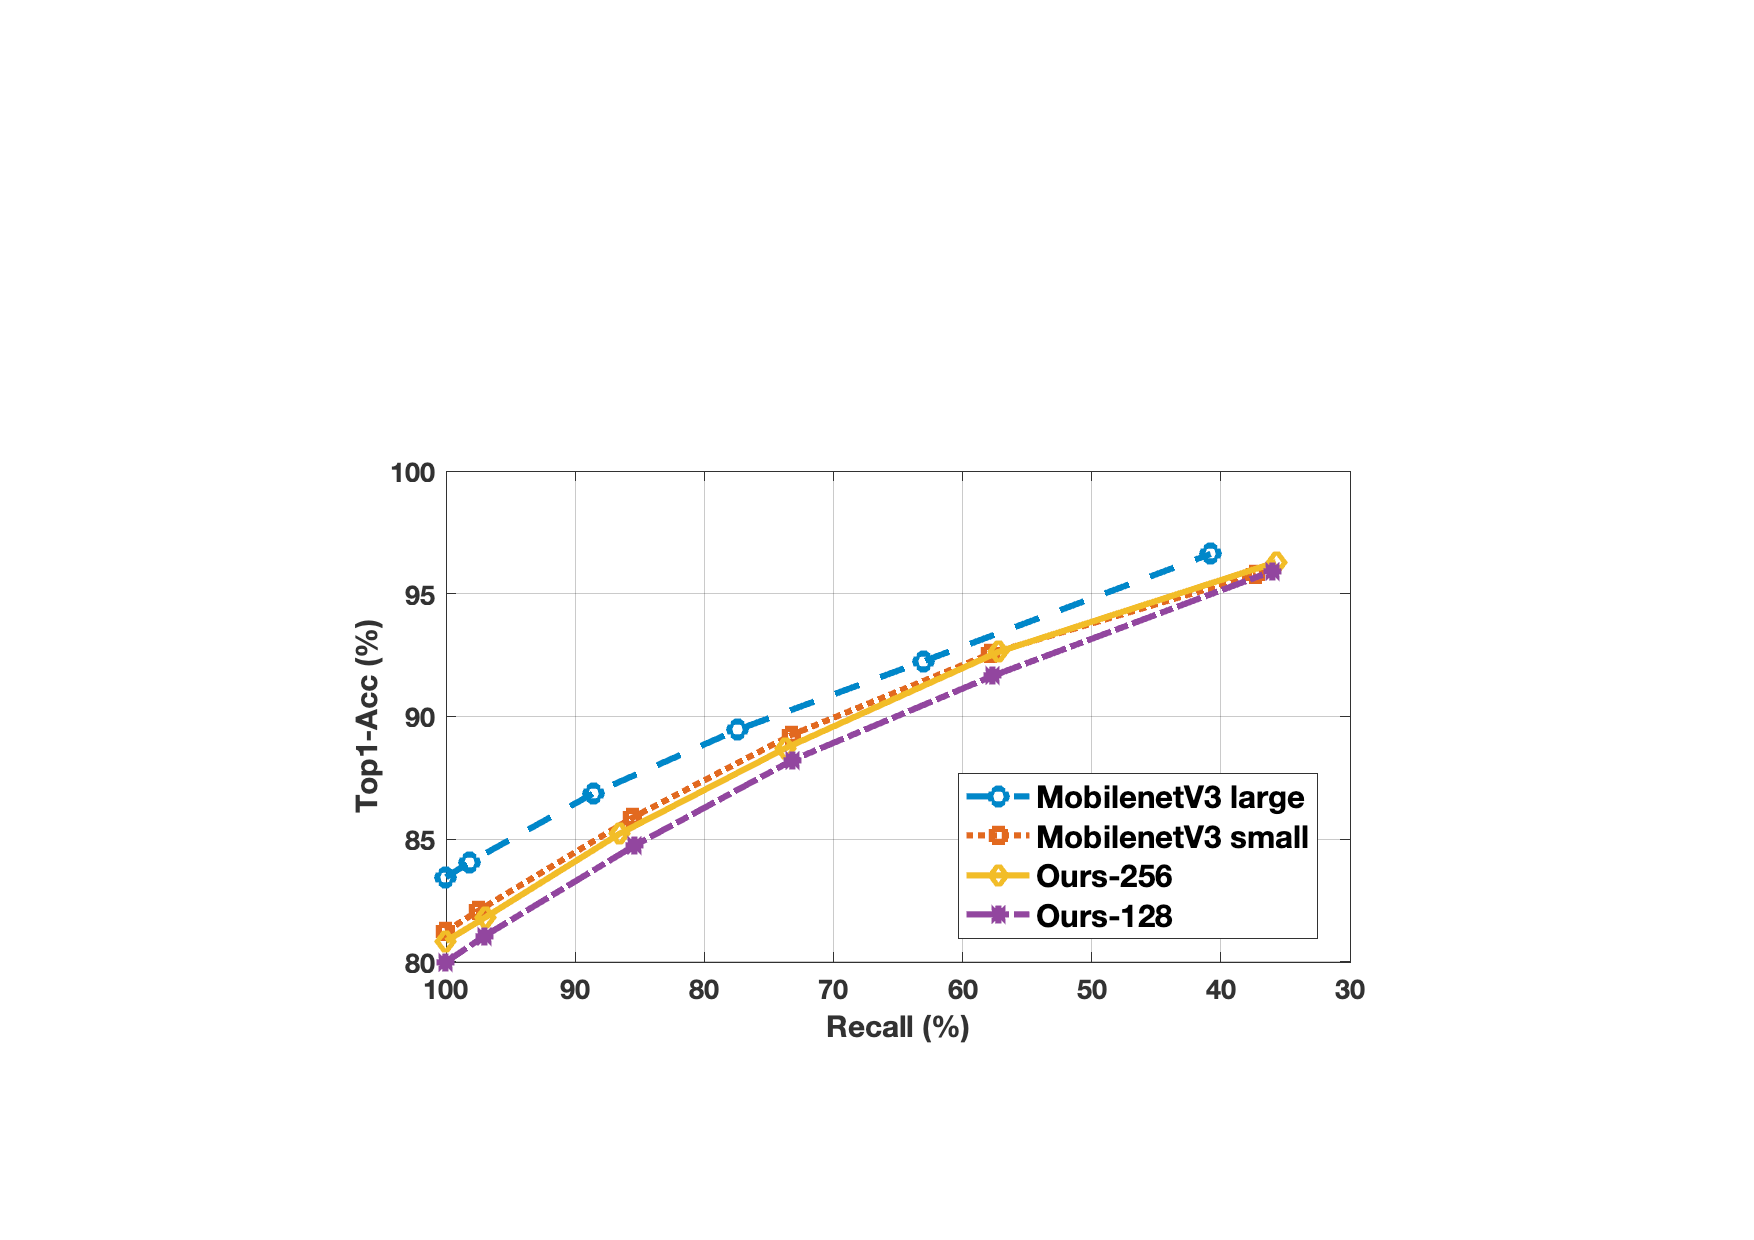
\includegraphics[width=0.45\textwidth]{fig/recall_dec.pdf}}
    \caption{The variation of recall versus accuracy. The thresholds are set as $[0, 0.5, 0.6, 0.7, 0.8, 0.9 ] $ successively.}
    \label{fig:recall_dec}
\end{figure}

In Fig. \ref{fig:recall_dec}, we explore the variation of accuracy versus changing of recall. We can find that as the recall decreases, the accuracy shows a linear increase approximately. When we use a threshold of 0.9, the final accuracy can exceed 95\%, but this reduces recall by a large margin. Since our tracking system does not rely solely on image information, and there will be multiple image results during a tracking session, we choose to balance 70\% recall to achieve 90\% accuracy.
In addition, we can also find that under the same threshold, \textit{ours-256} and \textit{MobilenetV3 small} perform closely, except that \textit{MobilenetV3 large} performs better.

\subsection{System evaluation}
To validate the effectiveness of the proposed method, we conduct 1) a experiment focusing on advance detection distance and 2) an ablation experiment to show the impact of each component on the detection system.
\subsubsection{Metrics}
To show the result intuitively, we introduce several metrics and provide the following statistics. The number of correct and advance detections is $n_{ac}$, and the number of total correct detections is $n_c$. $n$ describes the number of all detections.
For merics, we utilize $p_a$ to describe the percentage of advance and correct detections, which calculates through $\frac{n_c{}_a}{n}$. The total detection precision $p_t$ designed based on ERNet\cite{zhang2020elevated}, which calculates as $\frac{n_c}{n}$. And the average distance detected in advance $dist_a{}_v{}_g$ , which positive means the correct detection happened in advance while negative means it delayed. In addition, we use the precision of detection distance in several thresholds $k$ to show the performance.

\subsubsection{real-world detection experiment}
We conduct this experiment to verify the overall system performance by providing the statistics of the distance from the correct detecting location to the intersection. 

\begin{figure}[htbp]
    \centerline{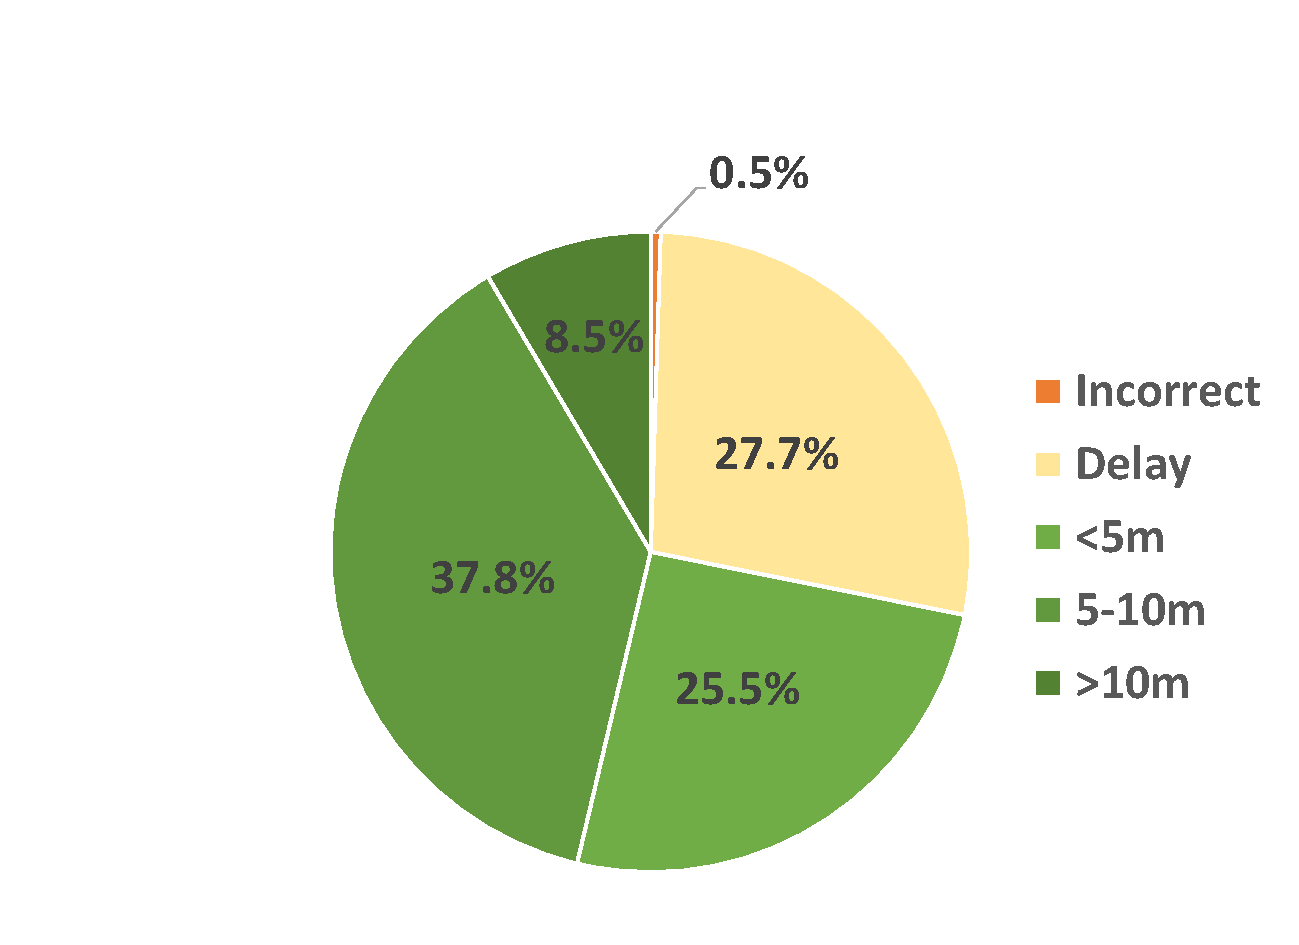
\includegraphics[width=0.45\textwidth]{fig/pie_chart.pdf}}
    \caption{Distance distribution from detection point to roads intersection point. $k$ is set as 5m and 10m.}
    \label{fig:pie_chart}
\end{figure}

As shown in Figure \ref{fig:pie_chart}, the correct yawing detection achieves 99.5\% and about 72\% of the correct detection happens in advance. 
Among them, the largest proportion appears in 5-10m, accounting for 37\% of the total, and about 8\% cases achieve more than 10 meters in advance.
We can see there are still some detections delaying, since the image results and IMU event results are accidental which cannot be ensured always exist and work. 

% In Figure \ref{fig:line_chart}, we explore the percentage of the correct detection versus distance between location and intersection. We can find that as the distance decrease, the precision of detection increases continuously. When the distance comes to 10 meters, the precision shows a steep increase and finally reaches about 80\%. 

\subsubsection{Ablation experiment}
This experiment shows the contribution of our two core components to the overall system by separating them and changing the combination with the basic map-matching method.

\begin{table}[htbp]
    \centering
    \caption{Ablation experiment}
      \begin{tabular}{c|c|c||c|c|c}
      \toprule[2pt]
      {GPS} & {Driving intention} & {IMU event} & {$p_a$} & {$p_t$} & {$dist_{avg}$} \\
      \midrule
       \checkmark& & & - & 93.8\% & -4.04m \\
       \checkmark& \checkmark & & 80.5\% & 100\% & 3.81m \\
       \checkmark& & \checkmark & 65.9\% & 97.9\% & 2.42m \\
       \checkmark& \checkmark & \checkmark & 89.6\% & 100\% & 5.11m \\
      \bottomrule[2pt]
      \end{tabular}%
    \label{tab:ablation}%
  \end{table}%

Table \ref{tab:ablation} shows the result as expected, the baseline method with only GPS data is unable to detect yawing in advance and have the worst performance, while adding image recognition data shows a remarkable improvement. Besides, the IMU event data helps to limit the impact of ambiguous data on the detection of pure GPS or image recognition, thus the proposed method gains the best result.

\section{Related Work}
When meeting a fork road, drivers are always confused about the planned route. Therefore, the detection of elevated and fork roads has become a hot topic in yawing detection research.

% Existing elevated detection methods mainly include Map-matching, Barometer-based, Feature-based and ERNet. 
Existing detection methods are mostly based on map-matching, barometer, feature and modeling GPS.
Lan Li \cite{li2012azimuth} proposed a map-matching method, which snaps a series of GPS points onto the map to estimate the trajectory of vehicles, and combine the GPS points with the azimuth of the vehicle to track the vehicle more precisely and detect whether it is yawing. Y. Gong et al. (2015) \cite{gong2015deel} proposed a feature-based method, which is based on the following four features: 1. Velocity variance; 2. Average number of tracked satellites; 3. Minimum Z-axis gravity component; 4. Z-axis linear acceleration variance. When people drive on the elevated road, the Z-axis gravity component of sensors will fluctuate, and the average number of tracking satellites will also change with the increase of altitude. So driving on the elevated road can be detected.The above two methods are affected by the GPS accuracy. M. Won et al. (2017) \cite{won2017hybridbaro} proposed a barometer-based method, which combines GPS data and smartphone barometer data. The air pressure on elevated road and surface road is different, so we can judge whether the vehicle is on an elevated. But air pressure is susceptible to speed. As the speed increases, the air pressure decreases. In addtion, not every device equips with barometer. Xiaobing Zhang et al. (2020) \cite{zhang2020elevated} proposed a neural network ERNet (Elevated Road Network) to identify whether a vehicle is driving on an elevated or not. This method inputs 4 high-level features into the neural network: 1. SPP; 2. group ID; 3. elevated road distance; 4 sequential speed to identify the road type through the output of the neural network. SPP refers to the distribution of satellite signals, which are very different between a vehicle on a surface road and on an elevated road. And the method divides roads into multiple groups for analysis. However, when GNSS data is missing, it will adversely affect feature 1, which in turn affects the output. The delay of the above four methods is relatively high, so that the yawing cannot be detected in time.
Moreover, \cite{kikuchi2014occluded} proposed a method to distinguish the side road from main road through image. It converts the images captured by the vehicle single camera into IPM images through the inverse perspective transformation method, and the road texture is used to determine whether there is a side road ahead. But it cannot detect whether the vehicle is yawing.

\section{Conclusion}
In this paper we introduced a novel framework to tracking vehicle on the fork road through image, IMU and GPS data. We designed a lightweight deep learning model to recognize the driver's intention when facing the fork. And we constructed a tracking system based on particle filter which combinated IMU event detection, image recognition and road information. 
Experiments in real-world datasets from our prototype have demonstrated the effectiveness.

\section*{Acknowledgments}
This should be a simple paragraph before the References to thank those individuals and institutions who have supported your work on this article.



% {\appendix[Proof of the Zonklar Equations]
% Use $\backslash${\tt{appendix}} if you have a single appendix:
% Do not use $\backslash${\tt{section}} anymore after $\backslash${\tt{appendix}}, only $\backslash${\tt{section*}}.
% If you have multiple appendixes use $\backslash${\tt{appendices}} then use $\backslash${\tt{section}} to start each appendix.
% You must declare a $\backslash${\tt{section}} before using any $\backslash${\tt{subsection}} or using $\backslash${\tt{label}} ($\backslash${\tt{appendices}} by itself
%  starts a section numbered zero.)}



%{\appendices
%\section*{Proof of the First Zonklar Equation}
%Appendix one text goes here.
% You can choose not to have a title for an appendix if you want by leaving the argument blank
%\section*{Proof of the Second Zonklar Equation}
%Appendix two text goes here.}



% \section{References Section}
% You can use a bibliography generated by BibTeX as a .bbl file.
%  BibTeX documentation can be easily obtained at:
%  http://mirror.ctan.org/biblio/bibtex/contrib/doc/
%  The IEEEtran BibTeX style support page is:
%  http://www.michaelshell.org/tex/ieeetran/bibtex/
 
 % argument is your BibTeX string definitions and bibliography database(s)
%\bibliography{IEEEabrv,../bib/paper}
%
% \section{Simple References}
% You can manually copy in the resultant .bbl file and set second argument of $\backslash${\tt{begin}} to the number of references
%  (used to reserve space for the reference number labels box).

% \begin{thebibliography}{1}
\bibliographystyle{IEEEtran}
\bibliography{mybib}

% \end{thebibliography}


\newpage

\section{Biography Section}
If you have an EPS/PDF photo (graphicx package needed), extra braces are
 needed around the contents of the optional argument to biography to prevent
 the LaTeX parser from getting confused when it sees the complicated
 $\backslash${\tt{includegraphics}} command within an optional argument. (You can create
 your own custom macro containing the $\backslash${\tt{includegraphics}} command to make things
 simpler here.)
 
\vspace{11pt}

\bf{If you include a photo:}\vspace{-33pt}
\begin{IEEEbiography}[{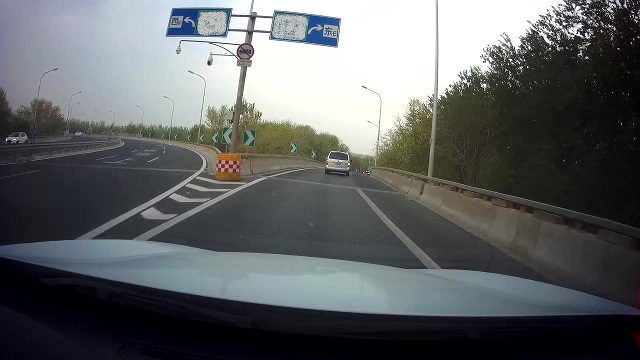
\includegraphics[width=1in,height=1.25in,clip,keepaspectratio]{fig/dashcam.jpg}}]{Michael Shell}
Use $\backslash${\tt{begin\{IEEEbiography\}}} and then for the 1st argument use $\backslash${\tt{includegraphics}} to declare and link the author photo.
Use the author name as the 3rd argument followed by the biography text.
\end{IEEEbiography}

\vspace{11pt}

\bf{If you will not include a photo:}\vspace{-33pt}
\begin{IEEEbiographynophoto}{John Doe}
Use $\backslash${\tt{begin\{IEEEbiographynophoto\}}} and the author name as the argument followed by the biography text.
\end{IEEEbiographynophoto}




\vfill

\end{document}


